\section{Aнализ литературно \\ патентных исследований}

\subsection{Обзор методов и средств тестирования сервоприводов}

Под сервоприводом в данной работе подразумевается вращающийся привод,
управляющий широтно-импульсной модуляцией, который за счёт обратной
связи позволяет точно контролировать вал сервопривода, поворачивая его
на заданный угол или поддерживая определенную скорость или ускорение.

Широтно-импульсная модуляция это метод модуляции сигнала, как
прямоугольной волны с переменной длиной между амплитудами.

Малогабаритные быстродействующие сервоприводы применяются в
современных высокоточных системах управления подвижными объектами:
рулевыми системами летательных аппаратов, автоматическими
манипуляторами, роботами с подвижными элементами конструкции и
др~\cite{dyakovSUBSTANTIATIONRELIABILITYSERVOMOTORS2023}.

В типичной системе контроля полета квадракоптера или дрона пять
параметров подлежат отслеживанию: длина четырех управляющих
сервоприводами импульсов, которые контролируют тягу, крен, тангаж и
рысканье, и напряжение питания.

В данной работе рассматривается система тестирования сервоприводов
квадрокоптера.  Назначение этой системы — тестирование отдельных
частей квадрокоптера, таких как сервоприводы,
блок управления скоростью или контроллер полёта ~\cite{Elector521}.

Говоря кратко, разрабатываемое изделие,
можно назвать одним общепринятым словом — сервотестер.

Сервотестер выполнен в виде платы, на которую, с помощью монтажа в
отверстия помещаются компоненты. Такой способ монтажа выбран для того,
чтобы облегчить сборку данной схемы, установку и смену тестируемых
компонентов или незначительного изменения схемы, необходимого для
взаимодействия с определенными компонентами, а также возможный ремонт.

В случае сложной конструкции, например при разработке полётного
контроллера, данный тестовый стенд позволяет наблюдать получаемый
сигнал на дисплее подключенном к микроконтроллеру сервтестера по
интерфейсу \textit{I2C} ~\cite{Elector521}.

\subsection{Анализ патентных исследований}

По своему характеру и содержанию патентные исследования относятся к
прикладным научно-исследовательским работам и являются неотъемлемой
составной частью обоснования принимаемых хозяйствующими субъектами
решений народнохозяйственных задач, связанных с созданием,
производством, реализацией, совершенствованием, использованием,
ремонтом и снятием с производства
объектов хозяйственной деятельности ~\cite{GOST-R-15.011-96}.

В~\cite{CN206161814U} представлена система тестирования сервоприводов,
включающая в себя главный компьютер, систему сбора данных, устройство
обработки данных, серводвигатель нагрузки, первый сервопривод и муфту.

Судя по всему один серводвигатель используется для тестирования
другого.

\begin{figure}[H]
  \centering
  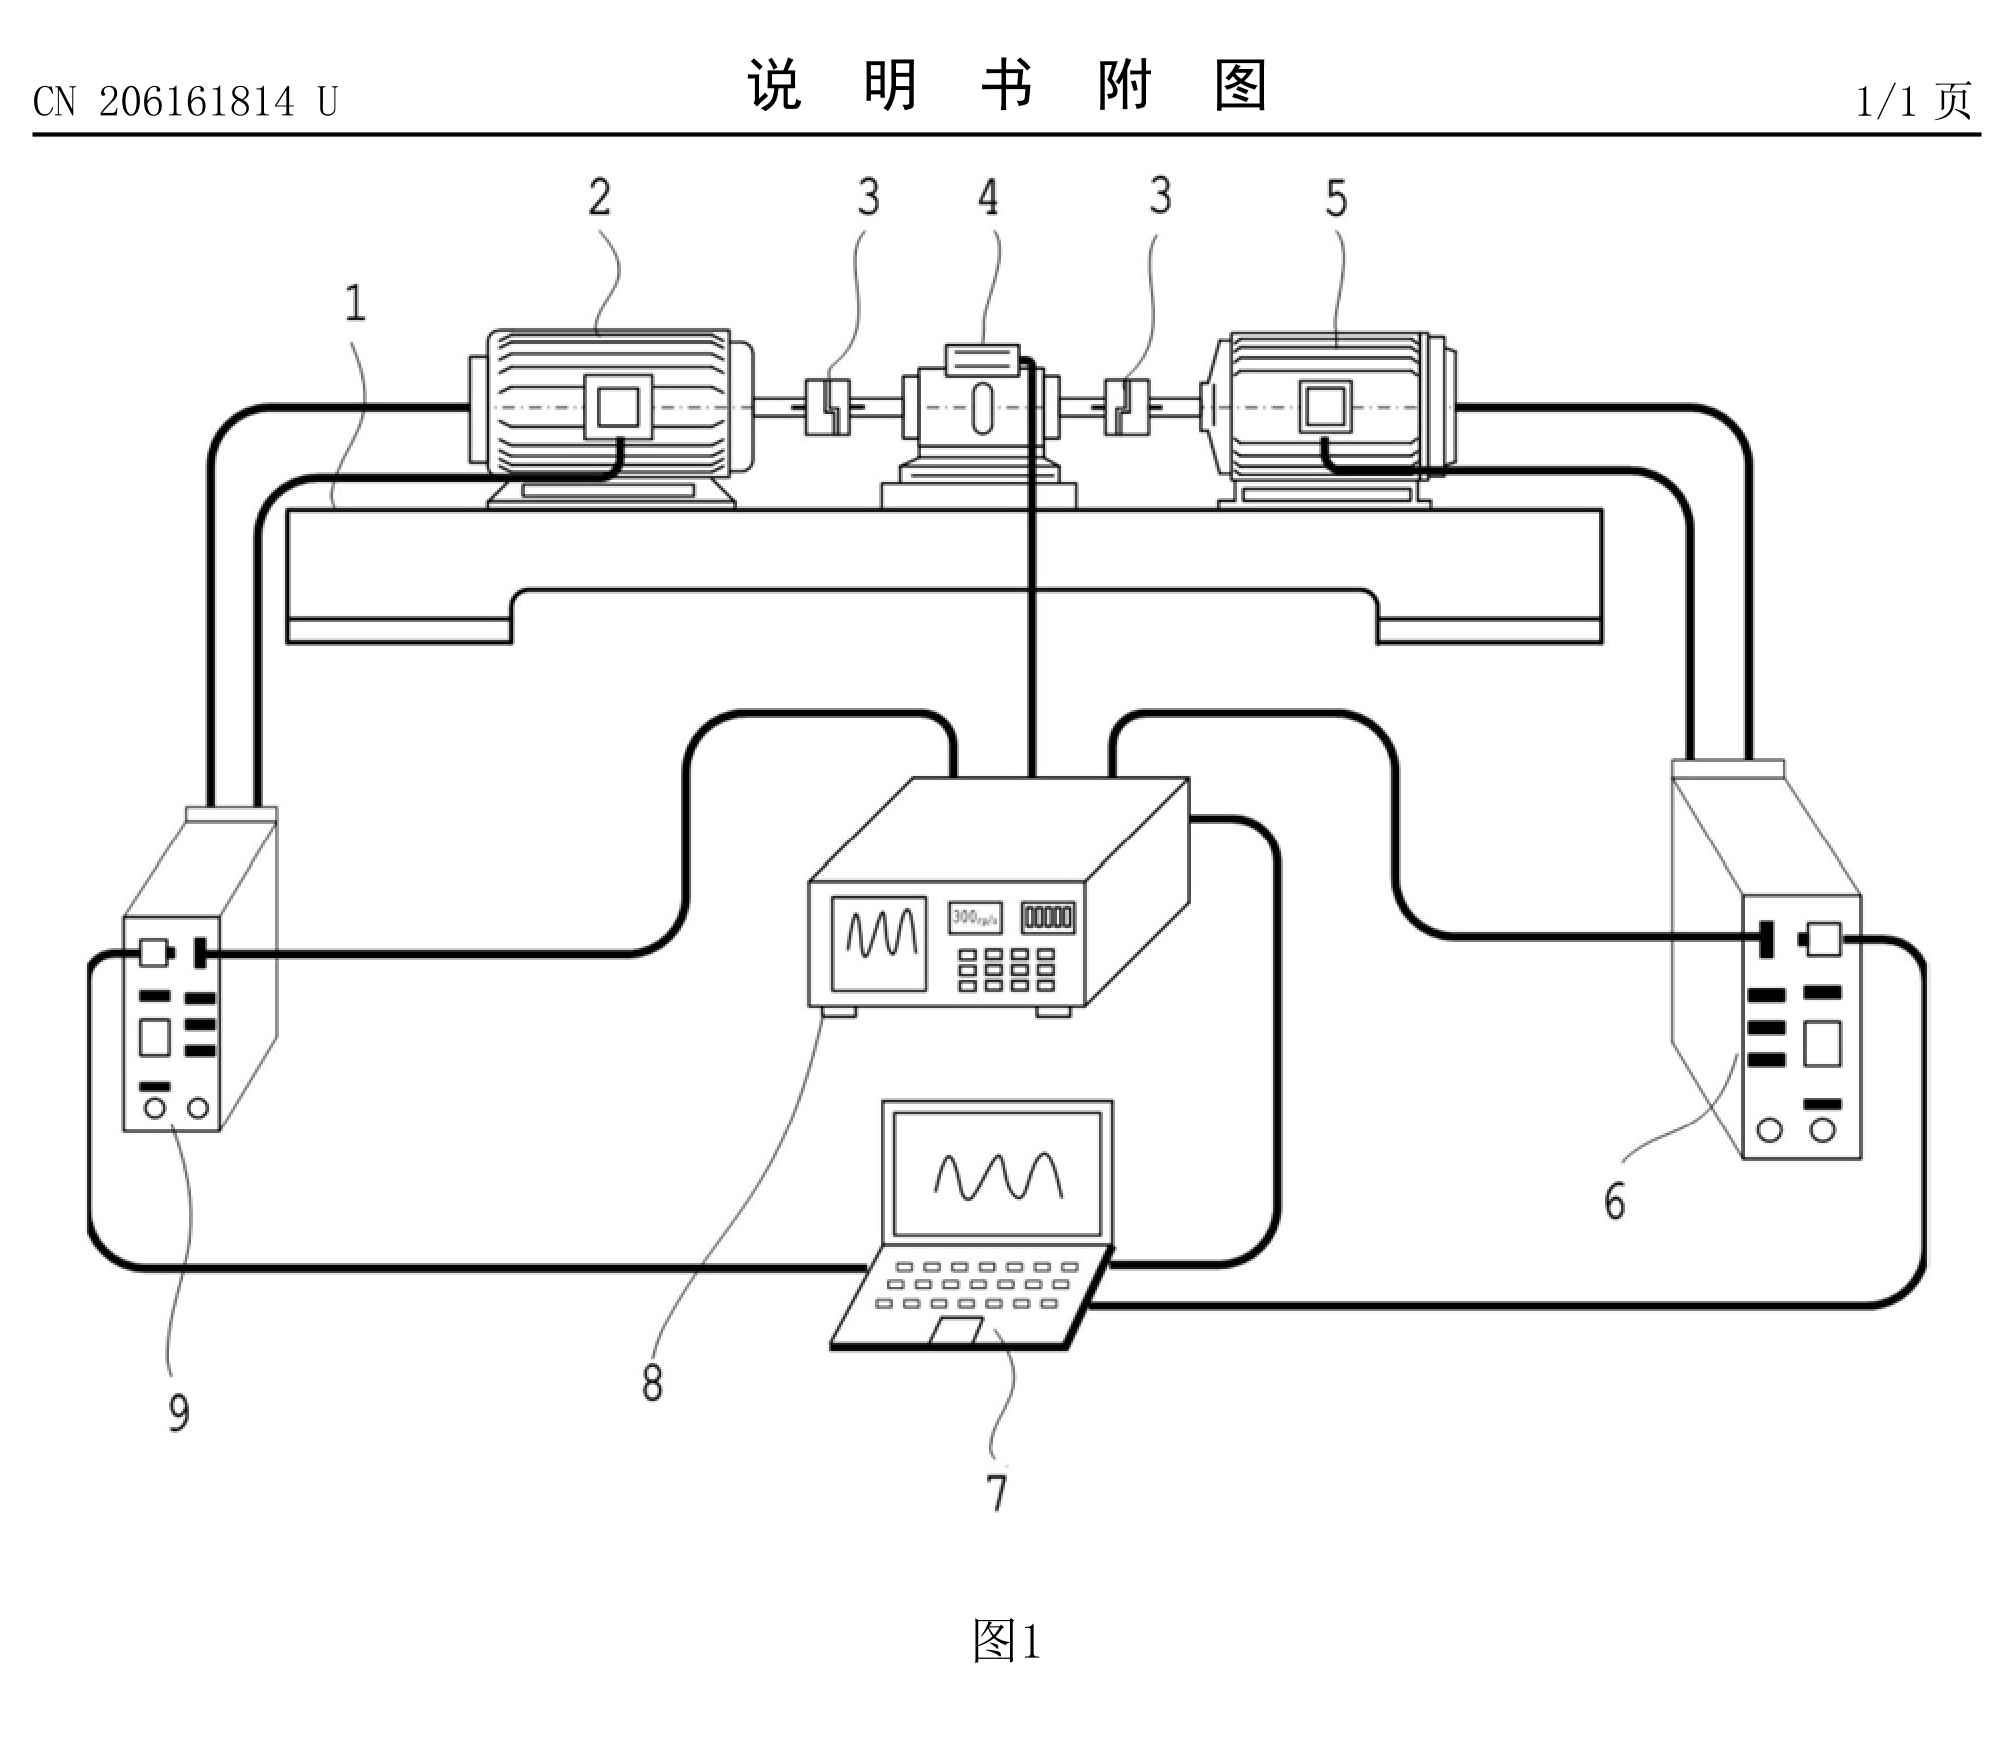
\includegraphics[scale=0.24]{CN_206161814_U.png}
  \caption{Изображение взятое из патента CN206161814U}
\end{figure}

Система проверки надежности серводвигателя включает в себя главный
компьютер (7), устройство сбора данных (4), устройство обработки
данных (8), серводвигатель нагрузки (2), первый сервопривод (9) и
муфту (3), при этом выходной вал серводвигателя нагрузки (2) соединен
с выходным валом испытываемого серводвигателя (5) через муфту (3) для
снижения шума; серводвигатель нагрузки (2) соединен с верхним
компьютером (7) через первый сервопривод (9), главный компьютер (7)
соединен с испытываемым серводвигателем (5) через второй сервопривод
(6).

Верхний компьютер (7) может управлять первым сервоприводом (9) и
вторым сервоприводом (6) для управления работой серводвигателя (5) и
серводвигателя нагрузки (2); устройство сбора данных (4)
соответственно подключено к выходному валу серводвигателя нагрузки (2)
и выходному валу испытываемого серводвигателя (5); устройство
обработки данных (8) соответственно с устройством сбора данных (4),
первым сервоприводом (9) и вторым сервоприводом (6).

В  ~\cite{CN108106873B} описывается не только система, но и метод исследования
сервоприводов на надёжность.

Сам метод оценки надёжности включает в себя следующие шаги:
\begin{enumerate}
\item Получить нагрузку от сервосистемы;
  % нагрузку (sensetive stress)
  
\item Для этой нагрузки найти предельные значения нагрузки для каждого
  компонента сервосистемы;
  
\item Определить испытательный диапазон для значений нагрузки и
  установить нагрузку для каждого компонента в соответствие с этим
  значением;
  
\item Каждый компонент по отдельности подвергается тесту на ускорение с
  соответствующими условиями для выяснения условий отказа и времени
  отказа по которому вычисляется средняя наработка между отказами (\textit{MTBF}).  
\end{enumerate}

Система для проверки надёжности сервоcистемы включает в себя:
\begin{enumerate}
\item Модуль сбора данных о нагрузке, используемый для сбора данных о
  значительном для сервосистемы механическом напряжении;
  
\item Модуль снижения механического напряжения, сконфигурированный для
  получения рабочих предельных значений напряжения каждого компонента
  сервосистемы;
  
\item Модуль определения условий испытания сконфигурированный для
  определения тестового диапазона механического напряжения,
  соответствующего каждому компоненту, в соответствии с рабочим
  предельным значением каждого компонента, и
  установки условия тестового напряжения каждого компонента в пределах
  тестового диапазона напряжения;
  
\item Модуль вычисления времени отказа используется
  чтобы каждого компонента по отдельности проводить испытания,
  с соответствующими ему условиями механического напряжения и вычислять
  среднею наработку между отказами в соответствии с временем отказа и
  условием отказа..
  
\item Компьютер, с памятью, процессором и программой записанной в
  памяти и исполняющийся на процессоре. Выполняющей испытания по
  вышеописанному методу.
  
\end{enumerate}

Вышеописанный метод и система используется для испытаний на надёжность
сервосистемы и выяснения того как время отказа отдельных компонентов
влияет на систему целиком.

% https://worldwide.espacenet.com/patent/search?q=pn%3DCN118549018A
В~\cite{CN118549018A} проводятся испытания cовмещающие испытания
сервопривода на крутящий момент и радиальную нагрузку на вал
сервопрвиода.

Система включает в себя:
\begin{enumerate}
\item Тормозное устройство;
\item Частотный преобразователь;
  % \item Нагрузка на котнролле % Load the controller
  
\item Cервоприводы;
\item Загрузочное устройство, включающее радиальный загрузочный узел и
  осевой загрузочный узел;
\item Силоизмерительное устройство, используемое для измерения
  крутящего момента и радиальной силы тестируемого внешнего двигателя;
  % \item Модуль ЦАП для сбора ана
  
\item Измерительное и контролирующие программное обеспечение
  совершающие анализ в реальном времени, обработка и храниене в реальном
  времни отслеживаемых данных и генерация детальных отчетов по
  исследованиям.
  1
\item Динамометрический двигатель, используемый для контроля выходного
  крутящего момента и управления крутящей нагрузкой внешнего
  тестируемого двигателя;
  
\item Таблица электрических параметров, используемая для измерения
  электрических сигналов на входе и выходе сервопривода и синхронного
  сбора сигналов крутящего момента и скорости с динамометрического
  двигателя; 
\end{enumerate}

Программное обеспечение для измерения и управления взаимодействует с
модулем ЦАП для управления выходной скоростью и крутящим моментом
аналогового сигнала внешнего тестируемого двигателя и управления
действием сервопривода.

В режиме управления крутящим моментом испытательная система возвращает
энергию и потребляет ее через тормозной блок или возвращает ее в
электросеть через инверторный блок преобразователя частоты, управляет
крутящим моментом на выходе динамометрического двигателя, управляет
крутящим моментом нагружаемого внешнего испытуемого двигателя и
представляет собой испытательную систему для проведения имитации
проверки рабочих характеристик внешнего испытуемого двигателяю.

Устройство измерения силы последовательно соединено с нагрузочными
концами радиального и осевого нагрузочных устройств, а также
подключено к контроллеру нагружения. Значение силы нагружения
собирается через датчик силы, и через контроллер нагружения
формируется замкнутый контур. Величина нагрузки радиального
нагрузочного устройства или привода осевого нагрузочного устройства
регулируется, и выполняется нагружение вала и радиальная сила внешнего
испытательного двигателя, и формируется испытательная система для
выполнения испытания надежности внешнего испытываемого двигателя.

% https://worldwide.espacenet.com/patent/search?q=pn%3DCN213842629U

В ~\cite{CN213842629U} система тестирования серводвигателей включает в себя
основание и микроконтроллер, на верхней поверхности основания расположены
соответвенно размещаемая и тестируемая детали.

Часть размещения включает опорную плиту и крепежную плиту, опорная
плита и основание параллельны друг другу, крепежная плита и опорная
плита перпендикулярны друг другу, а крепежное отверстие и вращающийся
вал соответственно предусмотрены на отверстии крепежной плиты;

Тестовая часть представляет собой тестер скорости вращения,
сигнализация расположена на верхней части тестера скорости вращения,
выходной конец сигнала тестера скорости вращения соединен с входным
концом сигнала одночипового контроллера, а входной сигнал сигнализации
соединен с выходным терминалом сигнала одночипового контроллера.

Используется тестер скорости, чтобы проверить, достигает ли скорость
серводвигателя номинальной. Если фактическая скорость ниже
номинальной, тестер скорости пошлет сигнал на микроконтроллер, а
микроконтроллер пошлет сигнал на сигнализацию, и сигнализация
оповестит персонал, что существует проблема с этим серводвигателем.

\begin{figure}[H]
  \centering
  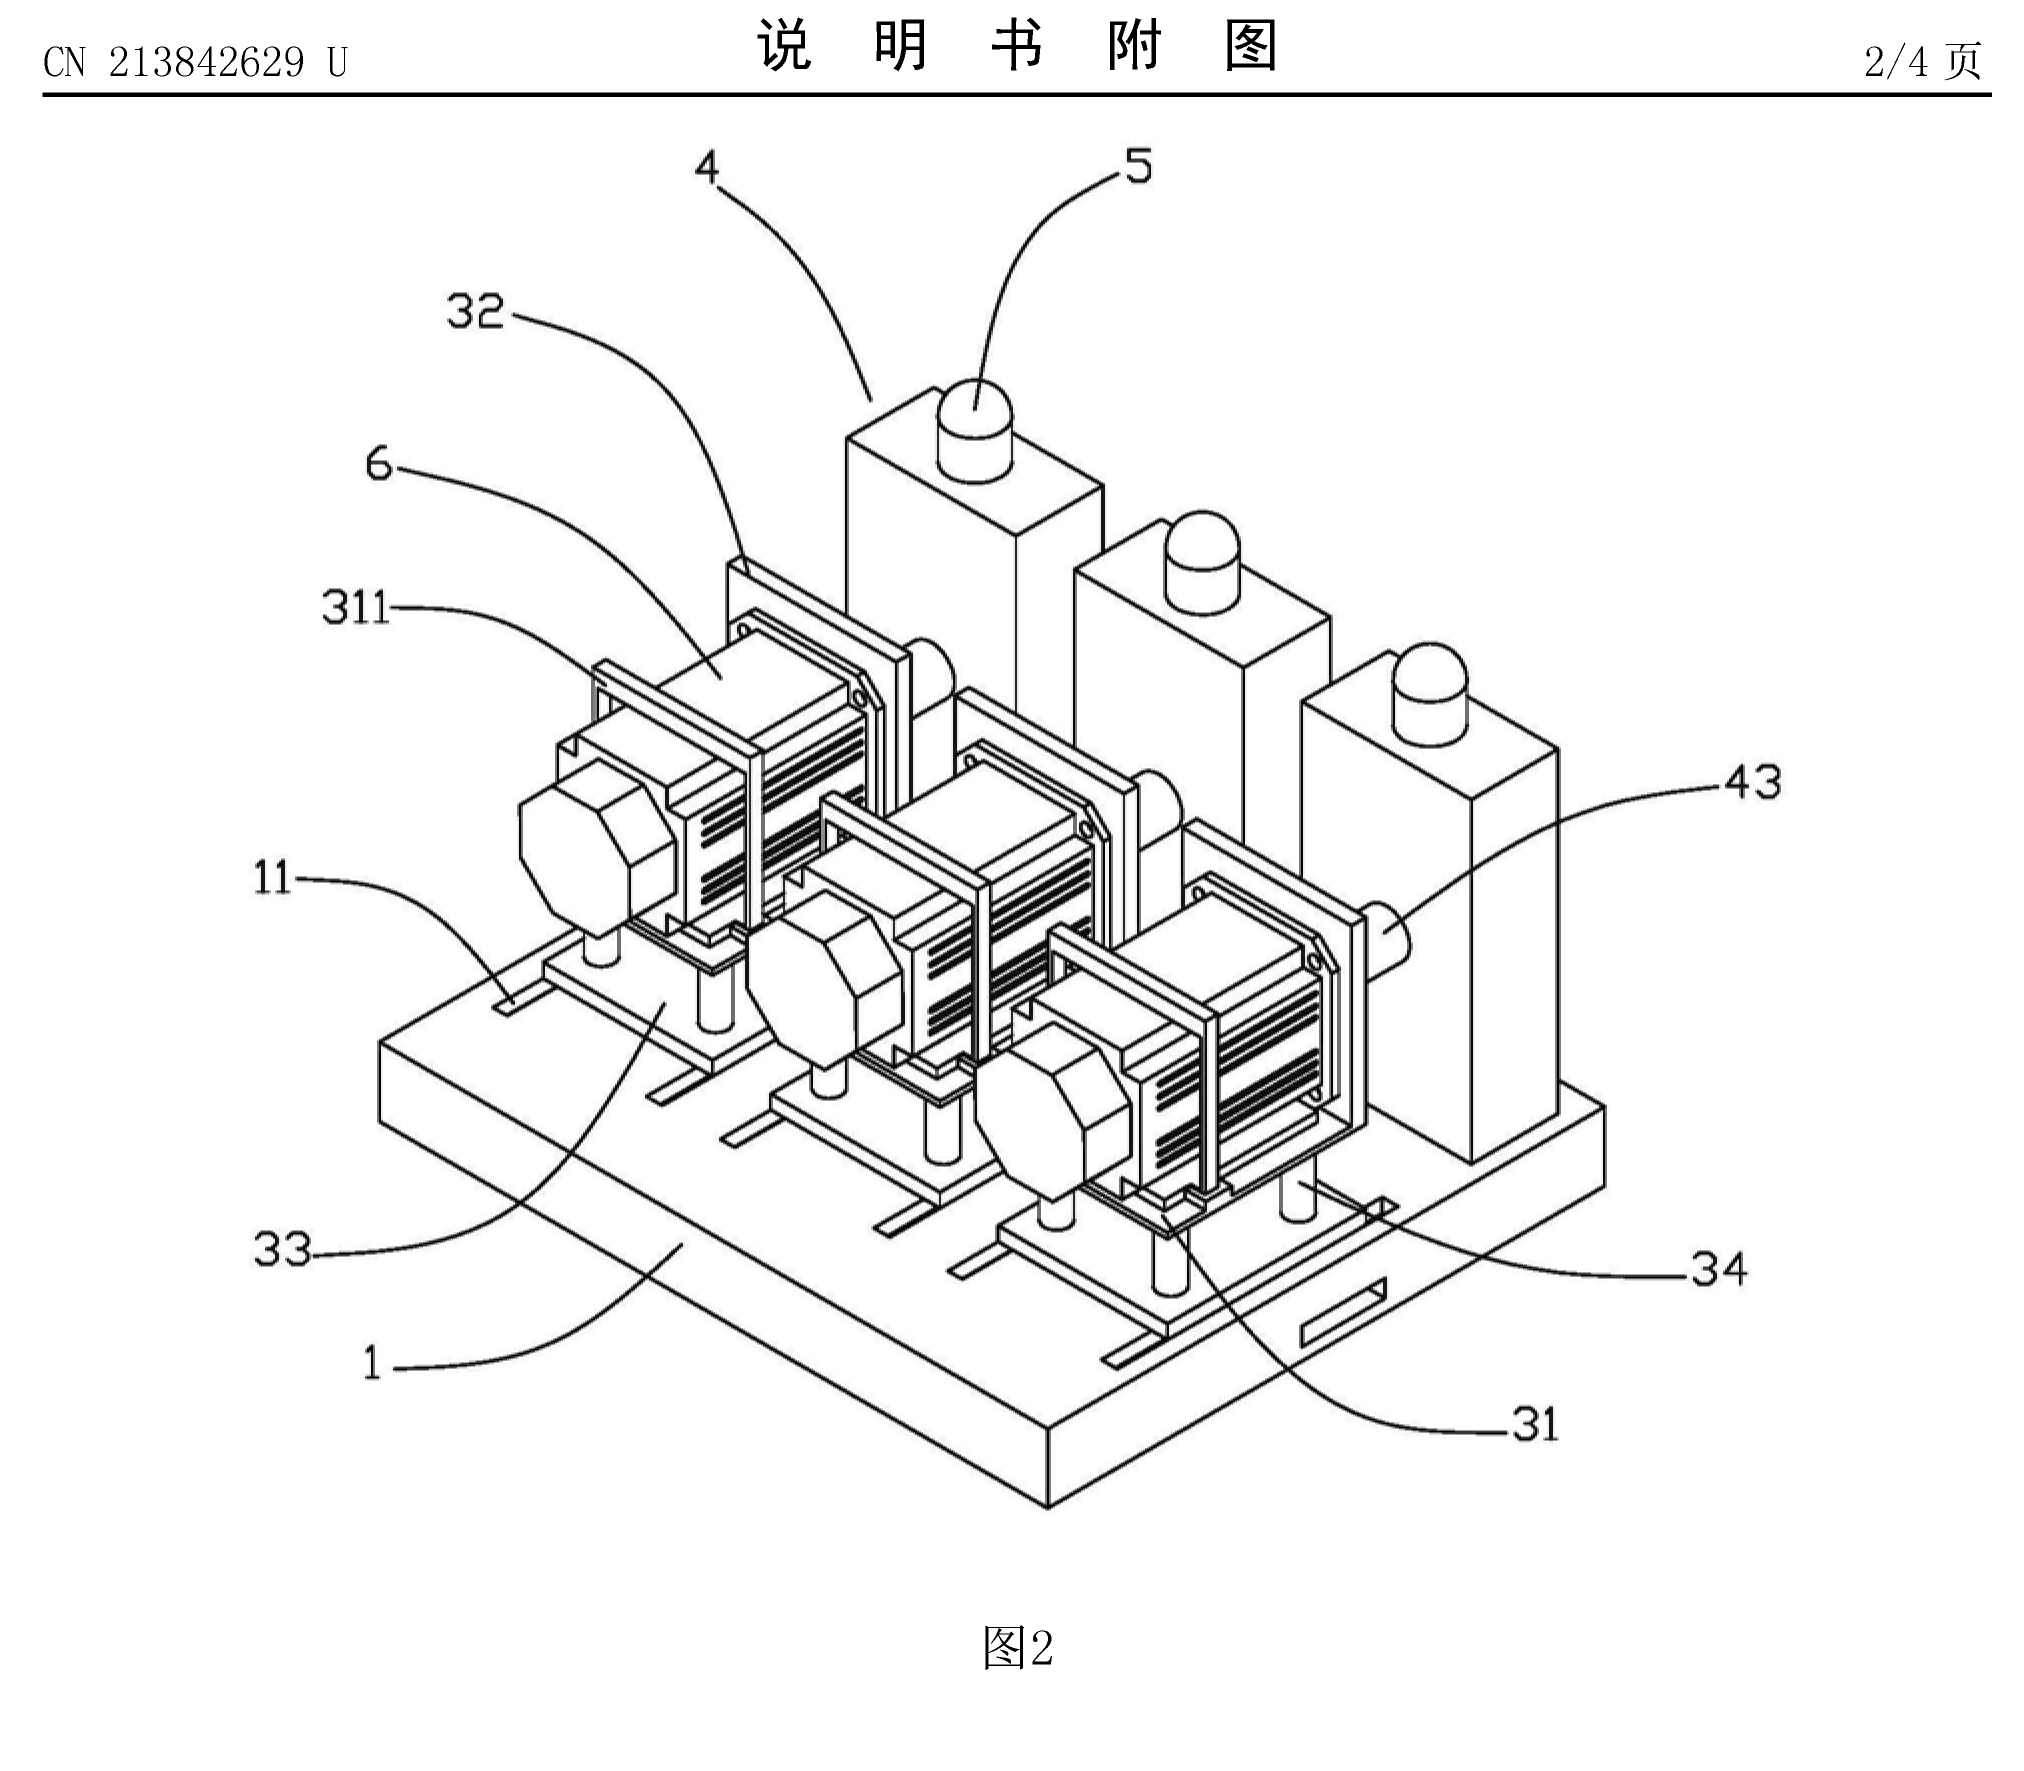
\includegraphics[scale=0.24]{CN_213842629_U.png}
  \caption{Изображение взятое из патента CN213842629U}
\end{figure}

На приведенном рисунке из патента можно видеть:
\begin{itemize}
\item Основание устройства (1);
\item Тестирующую часть (4);  
\item Сигнализаторы тестирующего устройства (5);
\item Серовпривод (6);
\item Скользящий рельс (11); 
\item Опорную плиту (31);
\item Неподвижный стальной ремень (311);  
\item Неподвижную плиту (32);
\item Подвижную плиту (33);  
\item Электрическую телескопическую штангу (34);
\item Втулку (43);
\end{itemize}

Рабочий кладет испытываемый серводвигатель (6) на опорную плиту (31),
совмещает монтажные отверстия на серводвигателе (6) с крепежными
отверстиями на крепежной плите (32) и закрепляет серводвигатель (6)
болтами, а затем закрепляет стальной ремень.  После установки (311)
электрическая телескопическая штанга (34) поднимается и опускается,
так что вал серводвигателя (6) совмещается с втулкой (43) тестера
скорости, затем электрический шкив приводится во вращение, заставляя
серводвигатель (6) приближаться к тестеру скорости, а вал
серводвигателя (6) вставляется в гильзу (43) тестера скорости и
заклинивается. Cерводвигатель (6) подключается к источнику питания,
вал приводит гильзу (43) во вращение, а фотоэлектрический выключатель
в тестере скорости проверяет скорость. Если скорость не достигает
номинальной скорости в течение времени, сигнализация (5)
предупреждает, и персонал может отметить серводвигатель (6), который
имеет проблему.

% https://worldwide.espacenet.com/patent/search?q=pn%3DCN210199269U

В ~\cite{CN210199269U} задачей полезной модели является создание
платформы для испытания серводвигателей, преимущество которой
заключается в повышении стабильности работы,
также перечислены несколько методом тестирования.

Платформа для испытания серводвигателей включает в себя раму и
нагрузочный двигатель, монтажная плита неподвижно соединена в раме,
монтажная рама неподвижно соединена на нижней поверхности монтажной
плиты, нагрузочный двигатель соединен под монтажной рамой болтами На
поверхности, выходная ось нагрузочного двигателя неподвижно соединена
с синхронным диском, монтажное отверстие проделано на монтажной плите
непосредственно в месте расположения синхронного диска, а верхняя
поверхность монтажной плиты соединена с подшипниковой плитой, на
подшипниковой плите открыто сквозное отверстие, сообщающееся с
монтажным отверстием, и синхронный диск используется для соединения с
выходным валом тестируемого серводвигателя.


\begin{figure}[H]
  \centering
  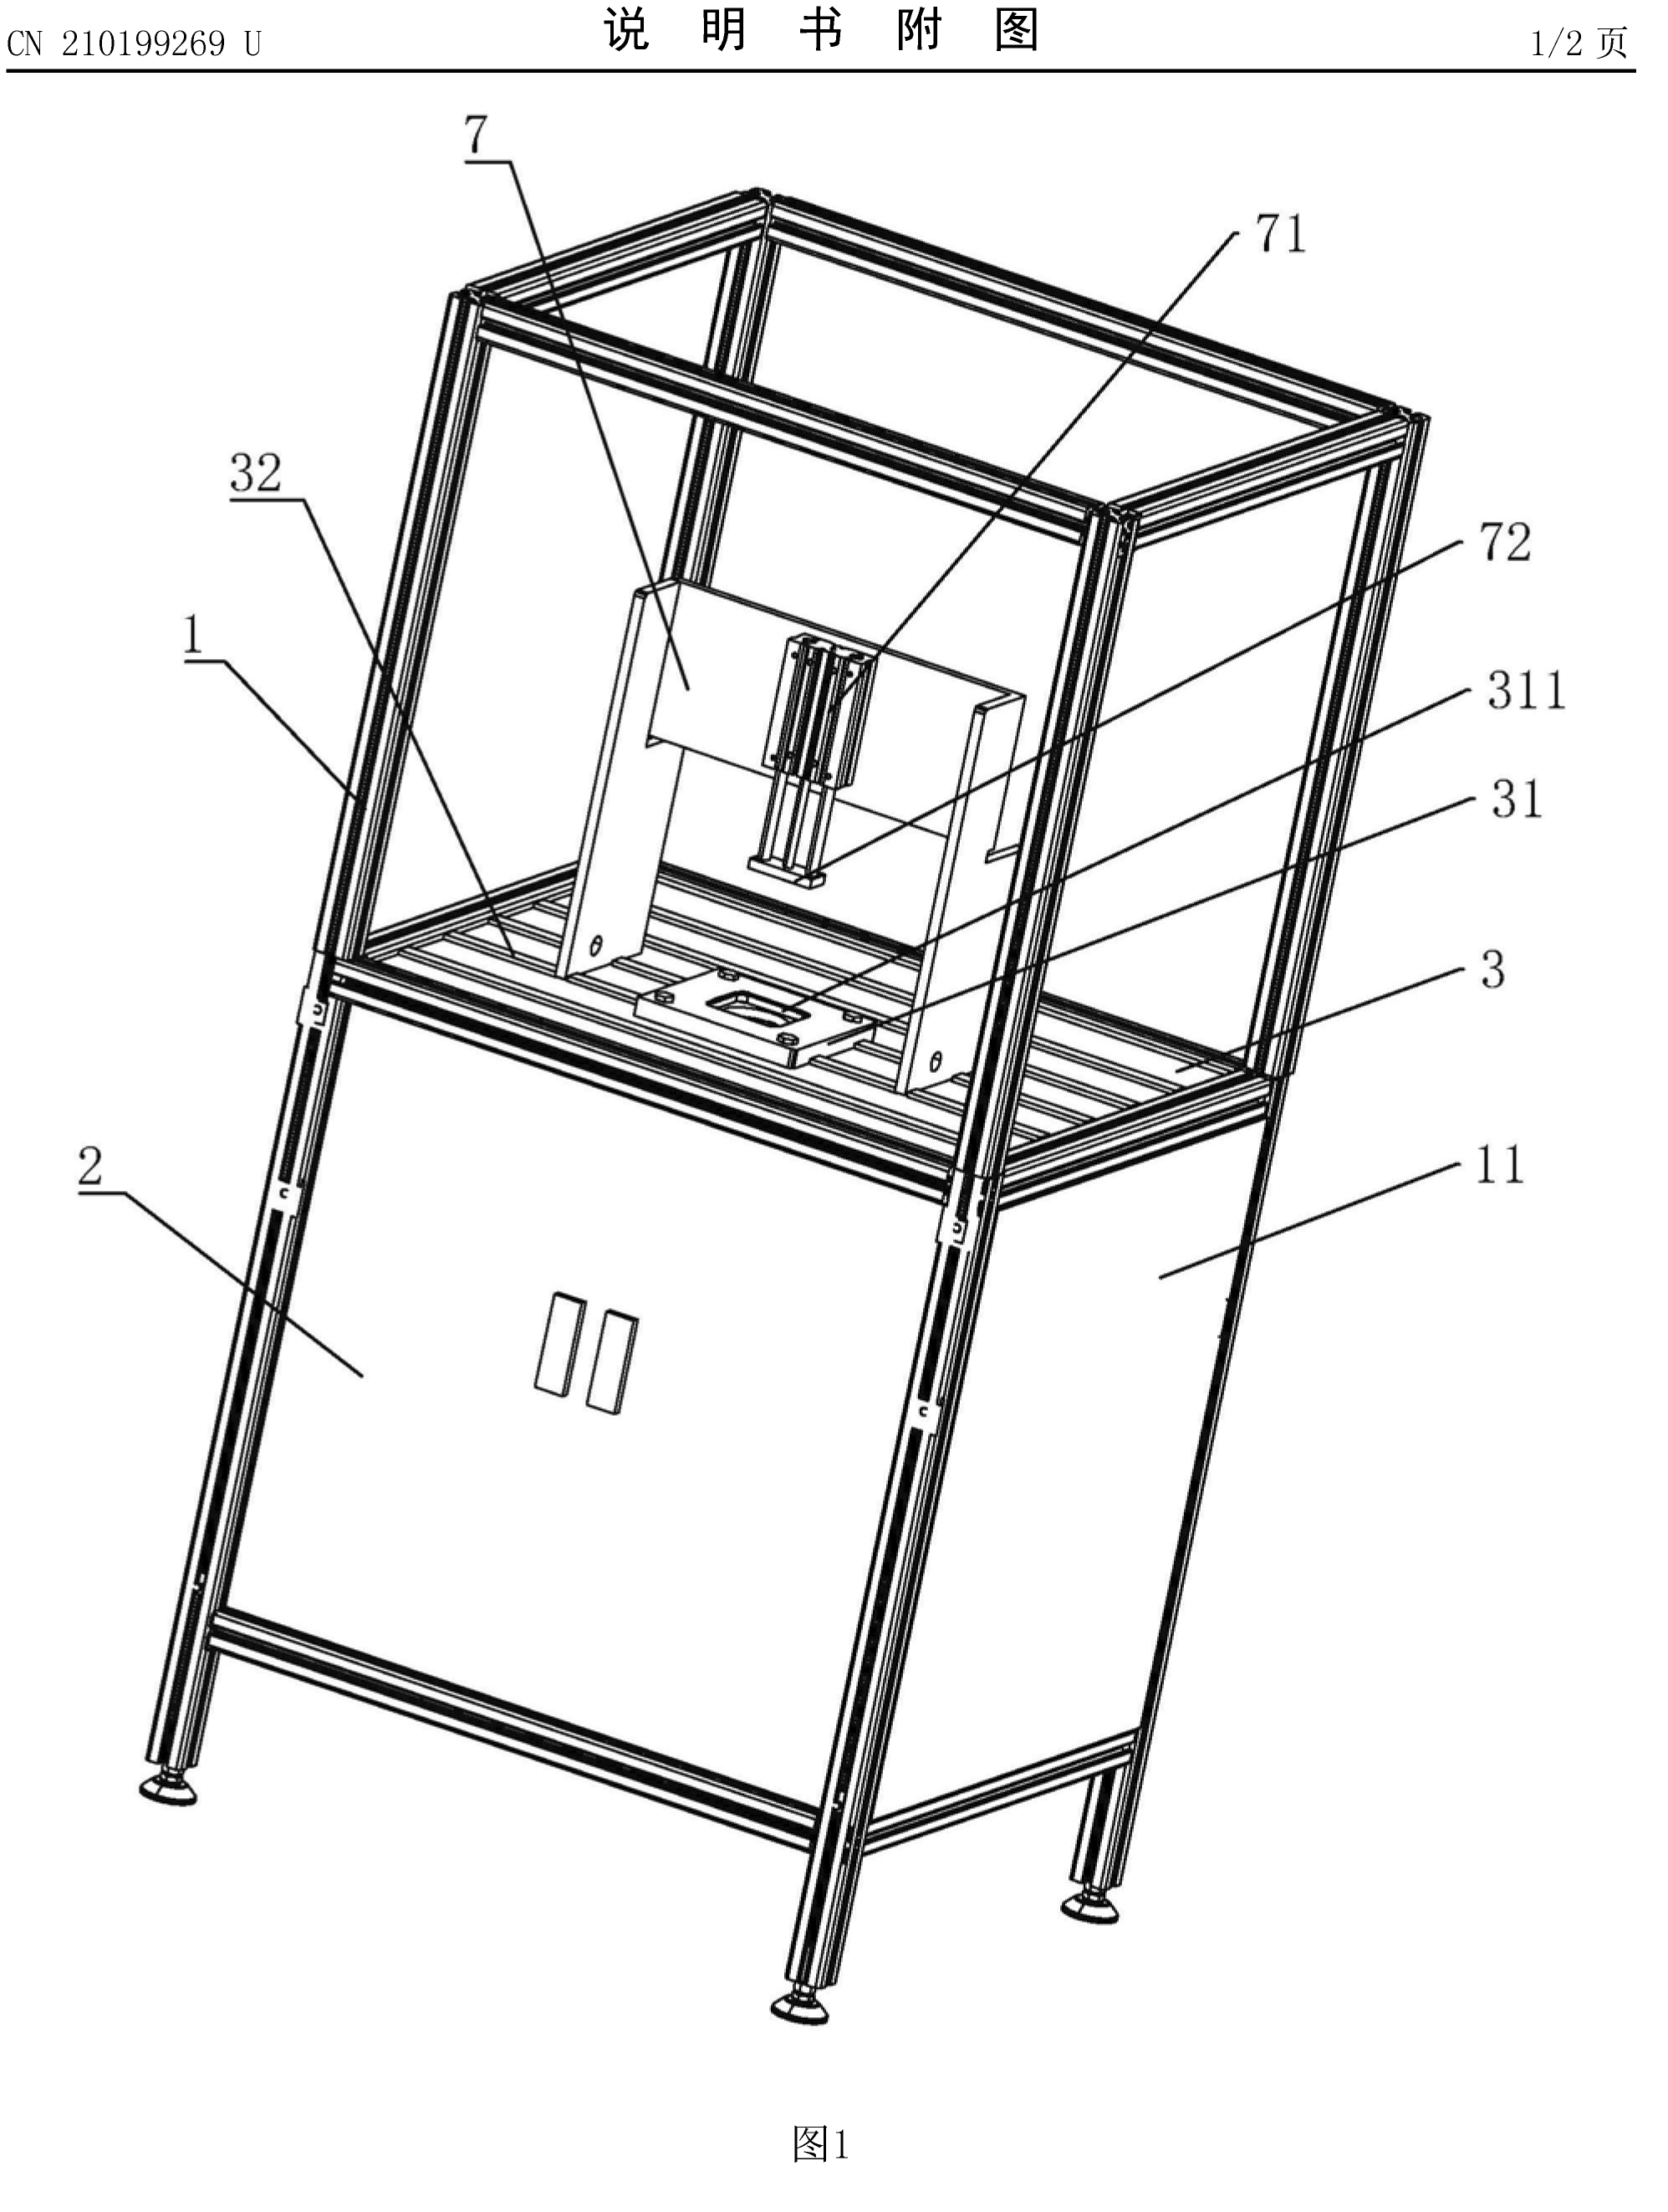
\includegraphics[scale=0.18]{CN_210199269_U.png}
  \caption{Cтруктурная схема воплощения настоящего изобретения;
    Изображение взятое из патента CN210199269U}
\end{figure}

На приведенном рисунке из патента можно видеть:
\begin{itemize}
\item рама (1);
\item защитная рама (11);
\item экранирующая дверь (2);  
\item плита для монтирования (3);
\item опорная плита (31);
\item центровочный паз (311);  
\item плита жесткости (32);
\item верхняя опорная рама (7);
\item цилиндр высокого давления(71);
\item нажимной диск (72);
\end{itemize}


В патенте приведено сразу несколько методов испытания сервопривода и
также отмечено, что это приведенный список испытаний не является
исключительным. По этой причине весь список методов провдения
испытаний был опущен.

Основные отличия разрабатываемой в данном работе системы заключаются в
следующем:
\begin{enumerate}
\item Устройство портативно. Не подразумевается монтаж на неподвижные опоры или основания;
  
\item Сервотестер проверяет только показатели непосредственно связанные с ШИМ
  сигналом подаваемом на входы сервоприводов;
  
\item Изделие использует один только микроконтроллер и не
  подразумевает подключения к ЭВМ или использования нескольких ЭВМ для вычислений;
  
\item Отсуствуют какие-либо строго оговоренные методы тестирования сервоприводов,
  которые применялись бы при работе сервотестера.
\end{enumerate}

В заключении остаётся добавить, что найденные при патентном поиске
изделия значительно отличались от разрабатываемого в данной работе
устройства.


\newpage

%%% Local Variables:
%%% mode: LaTeX
%%% TeX-master: "main"
%%% End:

